\documentclass[10pt,twocolumn,letterpaper]{article}

\usepackage{cvpr}
\usepackage{times}
\usepackage{epsfig}
\usepackage{graphicx}
\usepackage{amsmath}
\usepackage{amssymb}
\usepackage{mathtools}

\usepackage[shortlabels]{enumitem}

% Include other packages here, before hyperref.

% If you comment hyperref and then uncomment it, you should delete
% egpaper.aux before re-running latex.  (Or just hit 'q' on the first latex
% run, let it finish, and you should be clear).
\usepackage[breaklinks=true,bookmarks=false]{hyperref}

\cvprfinalcopy % *** Uncomment this line for the final submission

\def\cvprPaperID{group9} % *** Enter the CVPR Paper ID here
\def\httilde{\mbox{\tt\raisebox{-.5ex}{\symbol{126}}}}

% Pages are numbered in submission mode, and unnumbered in camera-ready
%\ifcvprfinal\pagestyle{empty}\fi
\setcounter{page}{4321}
\begin{document}

%%%%%%%%% TITLE
\title{Two Neural Algorithms of Artistic Style Transfer}

\author{Xingyu Chen\\
Columbia University\\
{\tt\small xc2416@columbia.edu}
% For a paper whose authors are all at the same institution,
% omit the following lines up until the closing ``}''.
% Additional authors and addresses can be added with ``\and'',
% just like the second author.
% To save space, use either the email address or home page, not both
\and
Ming Zhu\\
Columbia University\\
{\tt\small mz2655@columbia.edu}
}


\maketitle
%\thispagestyle{empty}

%%%%%%%%% ABSTRACT
\begin{abstract}
   The ABSTRACT is to be in fully-justified italicized text, at the top
   of the left-hand column, below the author and affiliation
   information. Use the word ``Abstract'' as the title, in 12-point
   Times, boldface type, centered relative to the column, initially
   capitalized. The abstract is to be in 10-point, single-spaced type.
   Leave two blank lines after the Abstract, then begin the main text.
   Look at previous CVPR abstracts to get a feel for style and length.
\end{abstract}


%%%%%%%%% BODY TEXT
\section{Introduction}

%-------------------------------------------------------------------------
\subsection{Motivation}
Artistic Style Transfer is to transfer the style of an image onto another image and get the synthetic, which is the combination of the style of the first image and the content of the second. Gatys \etal~\cite{Authors01} dealt with this problem through the application of covolutional neural networks. There are many researches and improvements based on the publication of Gatys \etal~\cite{Authors01}. Many of them try to make improvements since it is inefficient to go through the forward computation and backward propagation iteratively every time when there are new inputs, altough it can generate satisfying transfer results. 

To overcome the efficiency problem, Dmitry \etal~\cite{Authors02} and Justin \etal~\cite{Authors03} introduced the idea of generative network learning instead of one-time computation. Both of them utilized the representation features extracted by a pre-trained network and trained a feed-forward network. The network they trained is specialized for one style, which means for each style, there is a network to be trained. Zhang and Dana \cite{Authors04} improved the idea and designed a Multi-style Generative Network which is supportable for multiple styles. We then try to analyze how the improvements formed and compare their performance. 
%------------------------------------------------------------------------

\subsection{Work in this project}

In our project, we reproduce the algorithms introduced in Gatys \etal~\cite{Authors01} and Zhang and Dana \cite{Authors04} with PyTorch 0.4 framework. We compare the methods in these two paper, and analyze why they work and how the improvements come based on the experimental performance and results.


\section{Related work}

%-------------------------------------------------------------------------
\subsection{VGG network}
Simonyan and Zisserma \cite{Authors05} investigated the effect of depth on the accuracy of convolutional neural network for large-scale image recognition. The VGG-16 and VGG-19 they designed perform accurate on recognizing object in images. Both networks have small (3*3) convolutional filters and three fully connected layers. There are 13 and 16 convolutional layers in VGG-16 and VGG-19 respectively. It is nice that they public the values of parameters in the network for others to use. 

%------------------------------------------------------------------------
\subsection{Features representation}
Gatys \etal~\cite{Authors01} showed how to represent the content features and texture features of image in their paper. 

\textbf{Content features} indicate the objects in images, which can be represented as filter responses on $l$-th layer of the pre-trained recognition network. Assuming there are $Q_l$ feature maps on $l$-th layer, with size $H_l*W_l$ of each map. The content feature $F^l\in R^{Q_l*H_l*W_l}$. 

\textbf{Style features} show the texture of the images. Gatys \etal~\cite{Authors06} introduced the idea of feature space, which is actually Gram matrix among feature maps on $l$-th layer. Style features then can be represented as multi-scale Gram matrices on multiple layers. The Gram matrix explore the correlation between any two of the feature maps. Mathematically, the entry of Gram matrix on the $l$-th layer is the dot product of the $i$-th feature map and the $j$-th feature map. To facilitate calculation, the 2-dimension feature map is converted to 1-dimention vector.
\begin{align}
    G_{ij}^l= \sum_{k}{F_{ik}^l}{F_{jk}^l}
\end{align}


%------------------------------------------------------------------------
\section{Approach and Correctness}

\subsection{Style transfer algorithm \cite{Authors01}}
\noindent As referenced in Gatys \etal~\cite{Authors01}, the basic process of the algorithm is shown as follows.
\begin{enumerate}[a.]
    \item Initialize the output image $X$ as a random white noise image or the original content image.
    \item Feed the three input images into the pre-trained VGG network, which are original content image $C$, original style image $S$ and initialized output image $X$.
    \item Forward pass of the network. Compute the total loss which includes style loss and content loss.
    \begin{align}
    \mathcal{L}(C,S,X)_{\text{total}} &= \alpha \mathcal{L}(C,X)_{\text{content}}\nonumber\\ &+ \beta \mathcal{L}(S,X)_{\text{style}}
\end{align}
The content loss is computed between the feature maps $M^l$ of output $X$ and the feature maps $F^l$ of content image $C$ on some layer (assuming the $l$-th layer).
\begin{align}
    \mathcal{L}(C,X)_{\text{content}} = \frac{1}{2}\sum_{i,j}{(F_{ij}^l - M_{ij}^l)^2}
\end{align}
The style loss is total style loss computed on multiple layers. For each layer $l$, it is computed between the Gram matrix $N$ of output $X$ and the Gram matrix $G$ of style image $S$.
\begin{align}
\mathcal{L}(S,X,l)_{\text{style}} &= \frac{1}{4Q_l^2(H_lW_l)^2}\sum_{i,j}(G_{ij}^l-N_{ij}^l)^2\\
    \mathcal{L}(S,X)_{\text{style}} &= \sum_{l=0}^L w_l \mathcal{L}(S,X,l)_{\text{style}}
\end{align}
\item Backward propagation of the network. Compute the gradient of total loss with respect to the output image $X$ and update it.
\item Run the forward and backward pass for several epochs until the total loss is smaller enough.
    
\end{enumerate}


%-------------------------------------------------------------------------
\subsection{Multi-scale generative network \cite{Authors04}}
Multi-scale generative network (MSG-Net) consists of two parts which are 
Siamese Network and Transformation Network. In Siamese Network \cite{Authors07} design, there are two networks that share parameters. Each of them have their own inputs and their outputs will go through a loss function (or loss network) for model train. In the problem of style transfer, the two inputs are content image and style image respectively. Zhang and Dana \cite{Authors04} also introduced a special layer called CoMatch Layer that help build the relationship between the two models in Siamese Network. Thus, the output of Siamese Network would combine the style features of style image and preserve the semantic content of original content image. Transformation Network is for the upsampling of the output.


\noindent As referenced in Zhang and Dana \cite{Authors04}, the training process of the MSG-Net is shown as follows.
\begin{enumerate}[a.]
    \item Feed the content image $C$ and style image $S$ into the Siamese Network. Compute the Gram Matrix $G$ of feature maps of $S$ and combine them with the feature maps $F$ of $C$ on the $l$-th layer.
    \begin{align}
        \hat X^l = [F^l(C)^T W G^l(S)]^T
    \end{align}
    \item Upsample the output to recover the detail information from downsampled feature maps through upsampling residual block \cite{Authors08}
    \item The output that comes out of the above processes is similar to the output image that to be generated in section 3.1. The output and original content and style image then go through the loss network (the pre-trained VGG network). Next, compute content loss and style loss and update the parameters of MSG-Net backward based on the gradient of the loss.
\end{enumerate}


%-------------------------------------------------------------------------
\subsection{Implementation and reproduction}

Our implementation is based on PyTorch framework. The reproduction follows the process of the two algorithms we summarized from Gatys \etal~\cite{Authors01} and Zhang and Dana \cite{Authors04}. There are some implementation details.

When implementing the style transfer algorithm, we initialize the output $X$ as the original content image. Use VGG-16 network which has 13 convolutional layers and 3 max-pooling layers without connected layers. Choose feature maps on different layers as content representation and choose Gram matrices on different combination of layers as style representation. We will analyze according to the results.

When training MSG-Net, we initialize our network with customized number of generator filter channels and the pre-trained VGG-16 network. For each iteration, we minimize a weighted combination of the style and content differences of the generator network outputs and the targets for a given pre-trained loss network. Learning proceeds by sampling content images and style images and then adjusting the parameters of the generator in order to minimize the loss.

After the MSG network is trained, given a new content or style image, we just load the model and get the output image. 


%-------------------------------------------------------------------------
\subsection{Why works}
Both algorithms work depends largely on the pre-trained VGG network. VGG-Net \cite{Authors05} is a deep covolutional neural networks, which reaches 92.7\% accuracy when recognizing about 14 million images in 1000 categories. It is known that the input and all the intermediate layers could perform visual patterns after convolution with the filters. VGG-Net is used for object recognition, so during the process of training, the filters would be learned to capture the features that can represent object patterns and context information. Therefore, when inputs go through the pre-trained VGG-Net, the filter responses on each layer can display their content information in different level. That is why use feature maps as content representation.

Gram matrix explores the correlation between any two of the features. It eliminates the spatial information and does not concern the specific feature patterns. The non-diagonal entry represents the possibility that the two features exist together, and diagonal entry indicates the weight of the feature's appearance. Therefore, Gram matrix can represent the second-order statistics for the style features.


%-------------------------------------------------------------------------
\subsection{How improvements build up}
During the implementation, we find it takes about 30 seconds to transfer the style of an image onto the content of another with the algorithm in Gatys \etal~\cite{Authors01}. If there are 1000 style transfer tasks, it might need over 8 hours, which is sort of inefficient. Recall that the algorithm is taking two source images and the output image as input, and then update the output through the forward and backward pass of the pre-trained VGG-Net. That is, every time what it trains is the output image. It is naturally to think what if train a model instead of an image. Then the huge computation burden is taken to model training. Although it still needs time for updating the parameters of the model, the style transfer task can complete instantly with the trained model. Therefore, it is easier to understand the MSG-Net with CoMatch Layer and Upsample Convolution in \cite{Authors04}.


%------------------------------------------------------------------------
\section{Analysis of Results}


\subsection{Neural Style Transfer}

In this approach, we represent the content and style separably in the Convolutional Neural Network. Thus, in order to reproduce new result images, we can utilize both representations independently. To demonstrate our reproduction, we generate some results that mix the content and style representation from two different source images. For the content images, we use photograph taken by ourselves and from the Internet, and we use mainly photos of views, such as Columbia University and the Bund of Shanghai. For the style representations, we use  several famous artworks of different art styles.

\begin{figure}[t]
\begin{center}
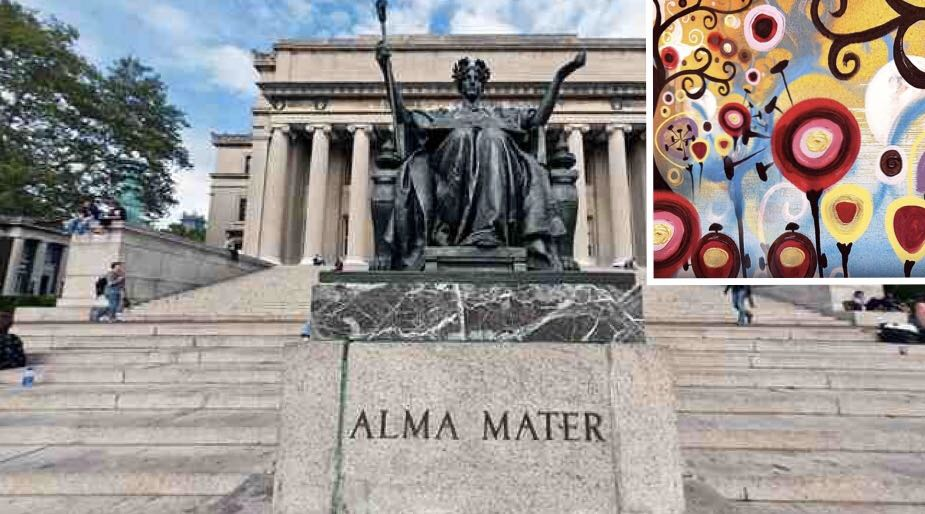
\includegraphics[width=0.6\linewidth]{images/columbia.jpg}
\end{center}
\caption{Columbia University as Content and Candy as Style}
\label{fig:long}
\label{fig:onecol}
\label{fig_col_candy}
\end{figure}

\begin{figure}[t]
\begin{center}
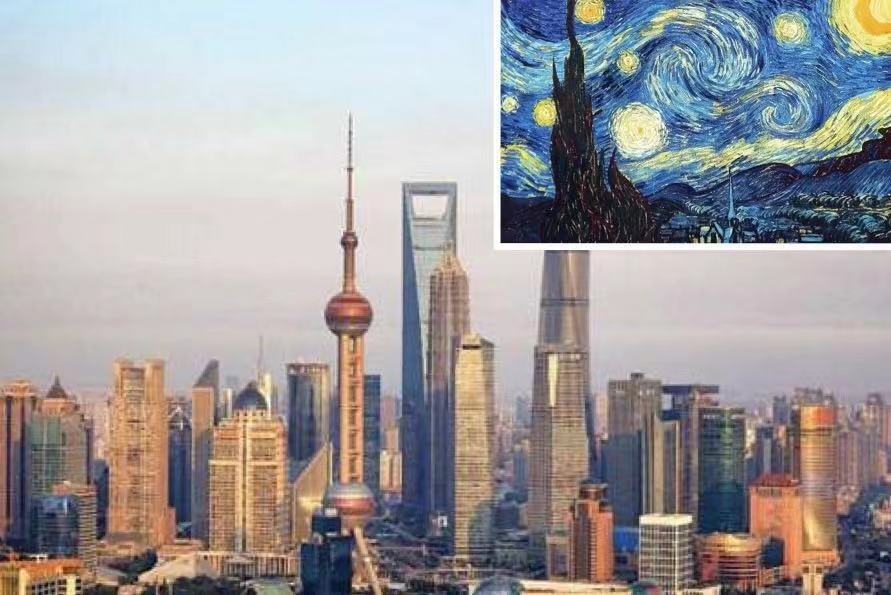
\includegraphics[width=0.6\linewidth]{images/shanghai.jpg}
\end{center}
\caption{Shanghai as Content and Starry Night as Style}
\label{fig:long}
\label{fig:onecol}
\label{fig_shn_star}
\end{figure}

First, we want to analyze the influence of different weight put on the content image and the style image. To achieve this we utilize different ratio of weight $\alpha / \beta$ to optimize the output image (see Equation (2)). The results is shown at Figure \ref{fig_ab}, where as the weight for content loss increasing, it is harder to see the style of the source artwork in the synthetic output. The output looks same with the source image when the ratio reaches 1000. 



\begin{figure}[t]
\begin{center}
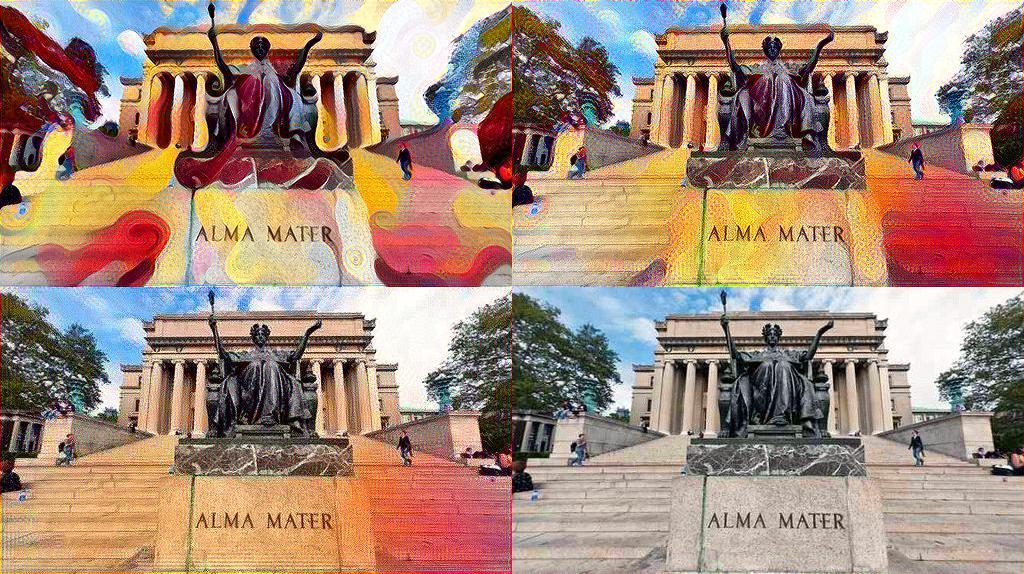
\includegraphics[width=0.9\linewidth]{images/merge_ab.jpg}
\caption{$\alpha/\beta=1.0,\text{ }10,\text{ }100\text{ and }1000$}
\label{fig:long}
\label{fig:onecol}
\label{fig_ab}
\end{center}
\end{figure}



Since we construct a multi-scale representation that includes multiple layers of the neural network to represent the style, the number and position of these layers determines the local scale on which the style is matched, leading to different visual experiences. We find that matching the style representations up to higher layers in the network preserves local images structures an increasingly large scale, leading to a smoother and more continuous visual experience. Thus, the visually most appealing images are usually created by matching the style representation up to high layers in the network. Figure \ref{fig_layers} shows the result comparison.

\begin{figure}[t]
\begin{center}
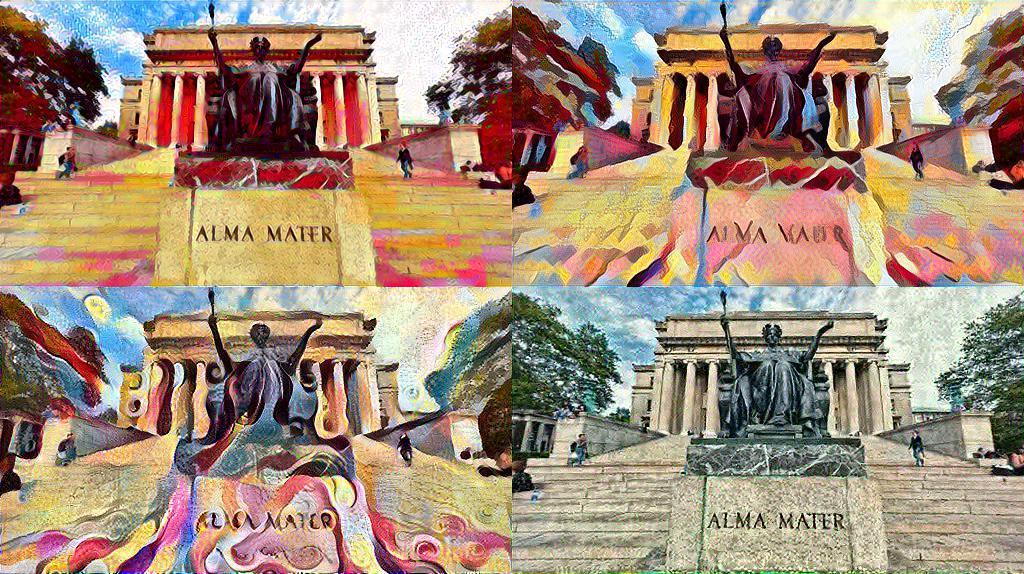
\includegraphics[width=0.9\linewidth]{images/merge_style.jpg}
\end{center}
\caption{Style Representation on Layer 1, 2, 3 and 4}
\label{fig:long}
\label{fig:onecol}
\label{fig_layers}
\end{figure}

\subsection{MSG network}

For the MSG network, we train the network for different epochs and then utilize them to produce new output images. The results of different training-level networks are shown in Figure \ref{fig_msg}.

\begin{figure}[t]
\begin{center}
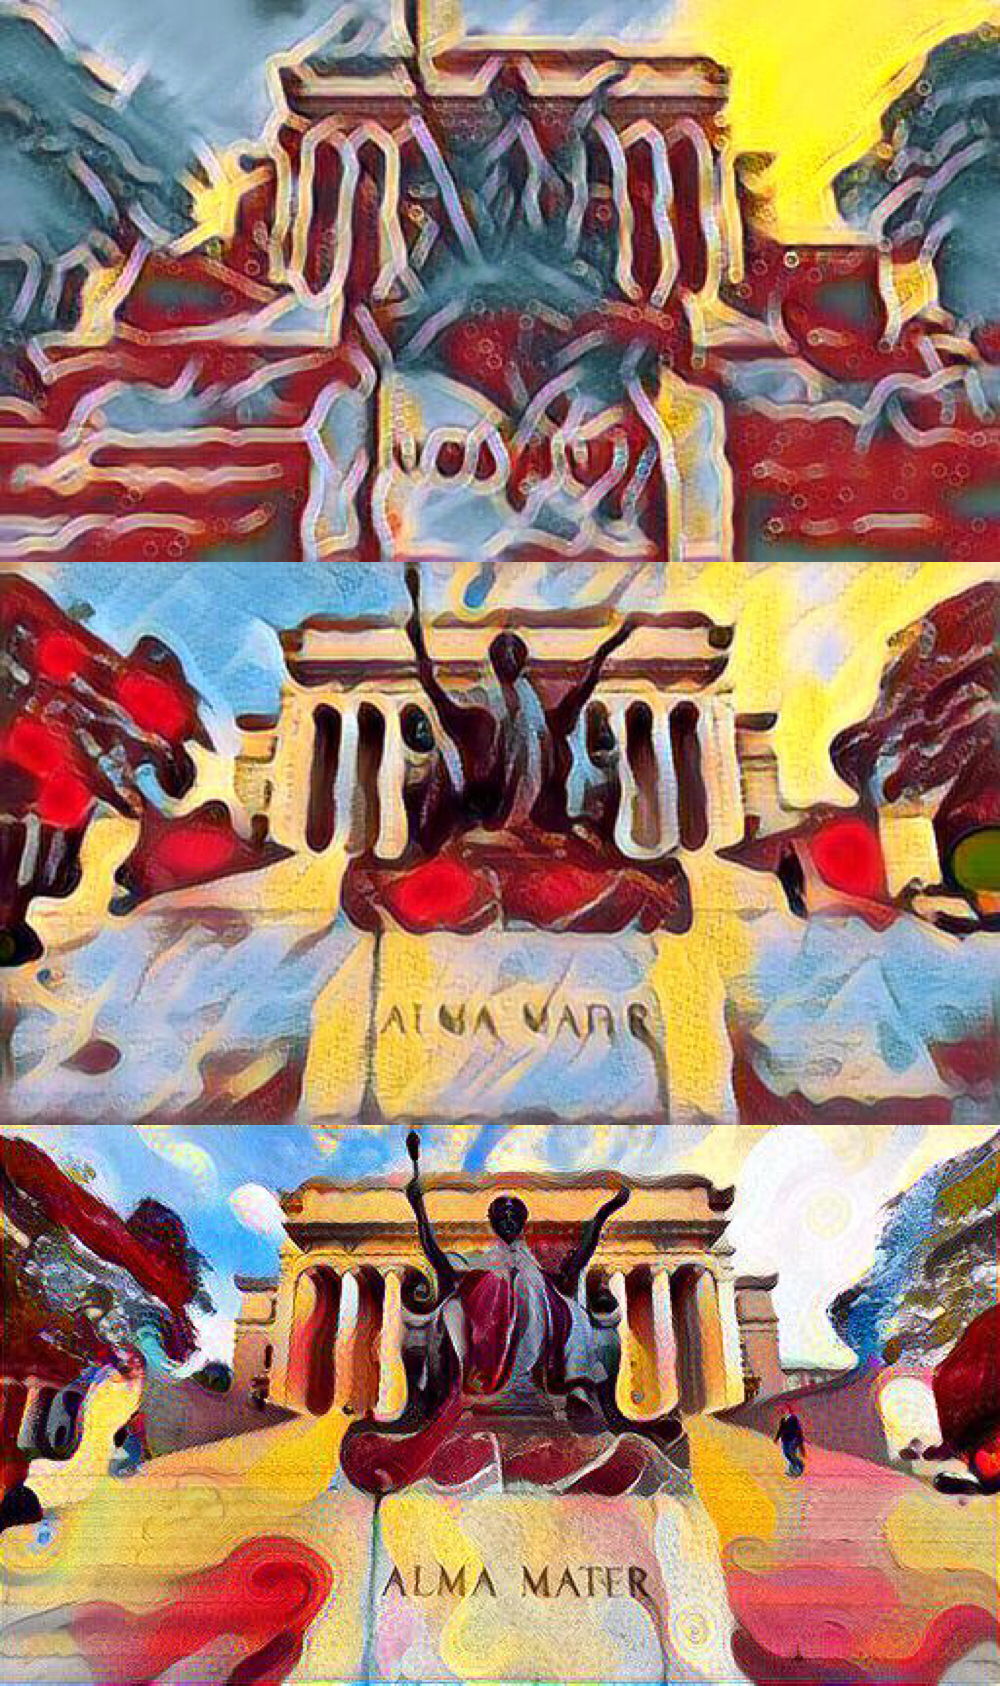
\includegraphics[width=0.6\linewidth]{images/msg_epoch_combine.jpg}
\end{center}
\caption{MSG Results for Network trained for 4, 8 and 20 Epochs}
\label{fig:long}
\label{fig:onecol}
\label{fig_msg}
\end{figure}

\subsection{Result Comparison}

We compare the result of these two approaches and the results are shown in Figure \ref{fig_col_cmp} and Figure \ref{fig_shn_cmp}.

\begin{figure}[t]
\begin{center}
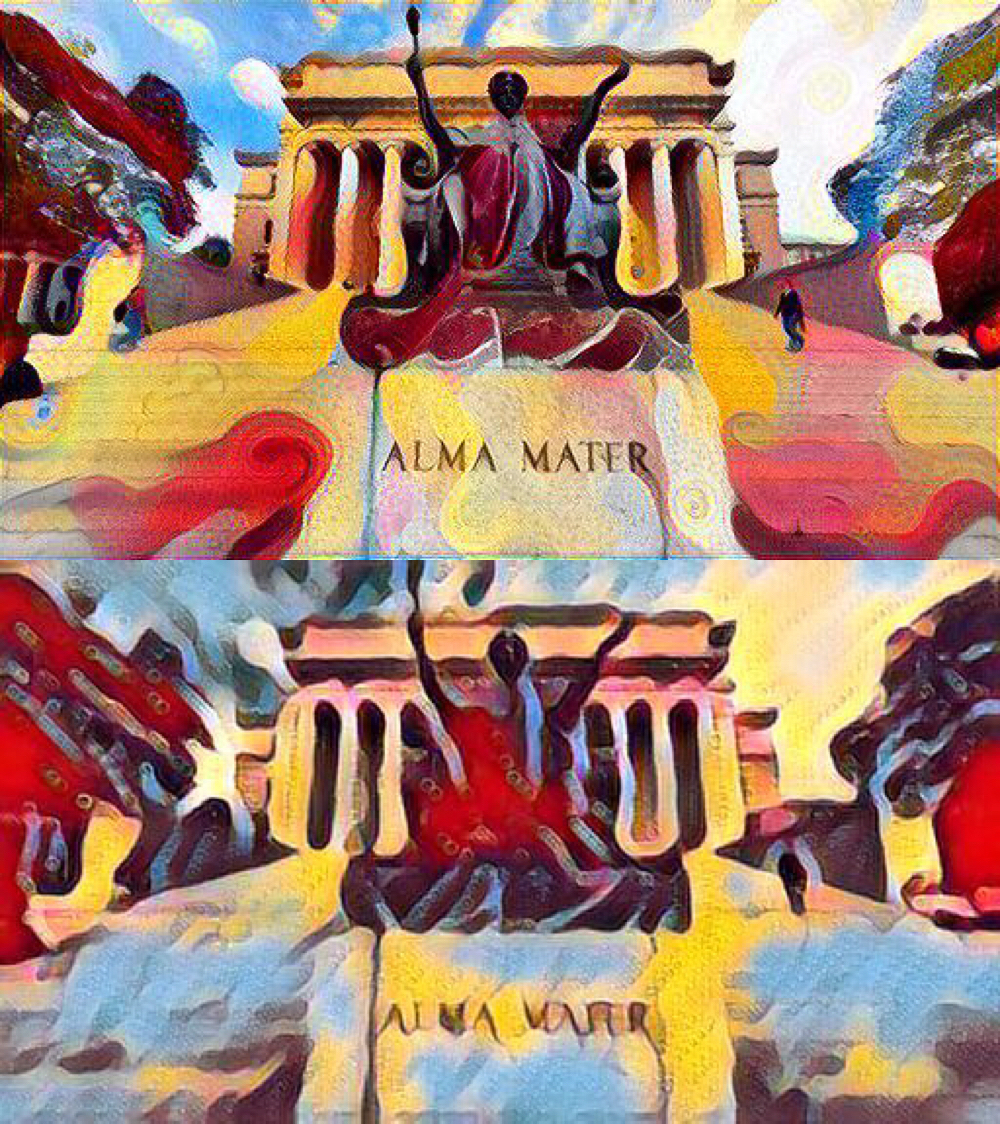
\includegraphics[width=0.6\linewidth]{images/col_cmp.jpg}
\end{center}
\caption{Neural Style and MSG Network Output of Columbia University and Candy}
\label{fig:long}
\label{fig:onecol}
\label{fig_col_cmp}
\end{figure}

\begin{figure}[t]
\begin{center}
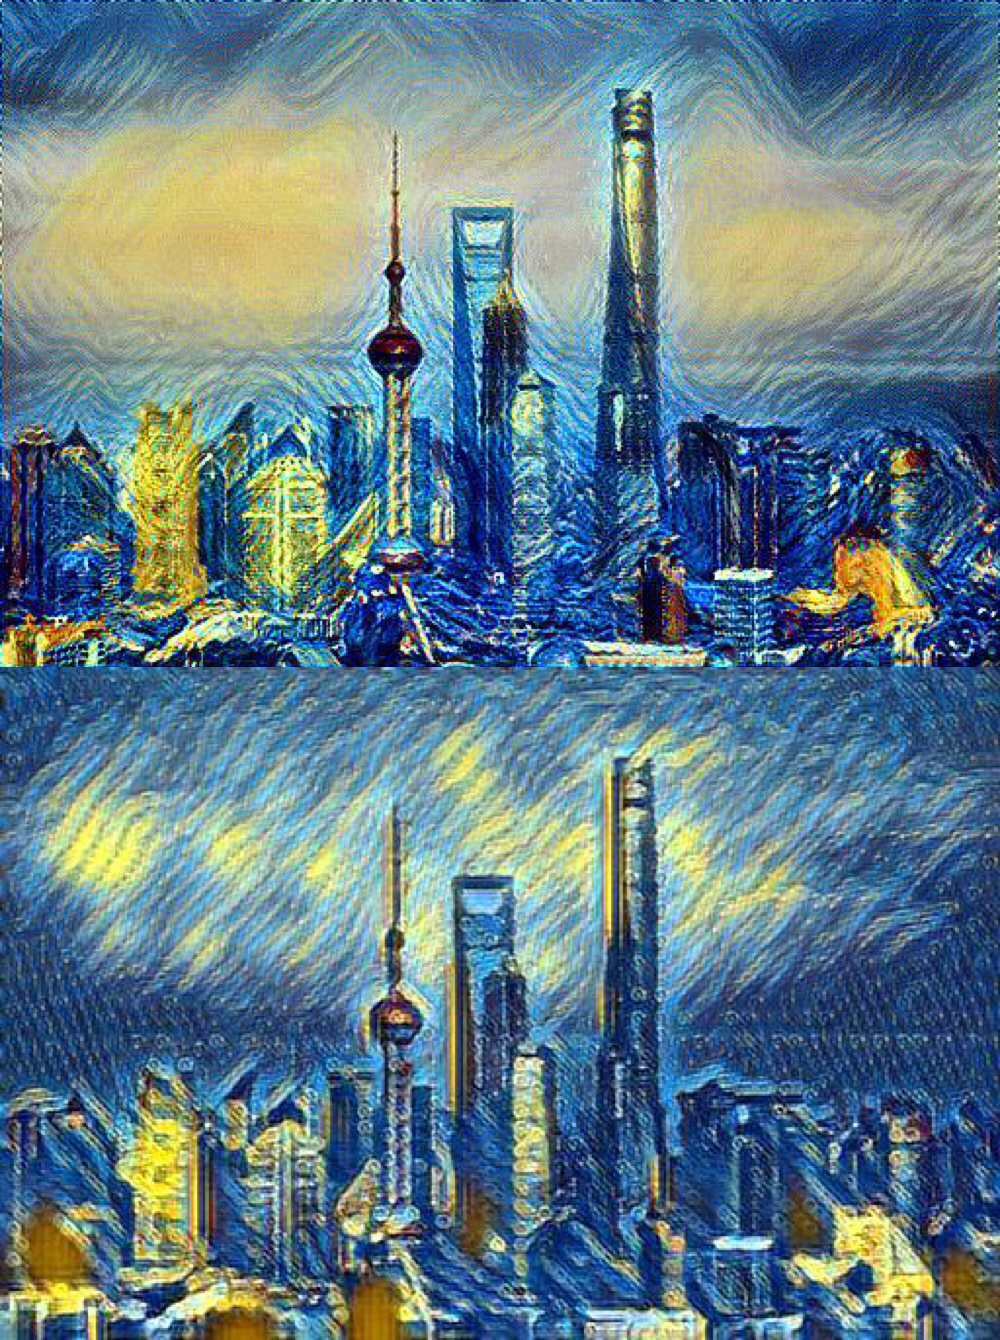
\includegraphics[width=0.6\linewidth]{images/shn_cmp.jpg}
\end{center}
\caption{Neural Style and MSG Network Output of Shanghai and Starry Night}
\label{fig:long}
\label{fig:onecol}
\label{fig_shn_cmp}
\end{figure}

\subsection{Transfer Efficiency}
It takes 17-29 seconds to complete style transfer with the algorithm in \cite{Authors01}, while it takes 1-3 seconds to style transfer with the MSG-Net in \cite{Authors04}. Apparently MSG-Net is more efficient than style transfer algorithm. 



\section{Clarity and Reproducibility}
Our code resides in \newline $https://github.com/stellarnull/cv\_proj$.


\section{Division of work}
Xingyu Chen is responsible for the train and evaluation of MSG-Net. She also do the analysis for the performance of Style transfer algorithm and MSG-Net.

Ming Zhu is responsible for the implementation of style transfer algorithm. She summarize the process of algorithms from Gatys \etal~\cite{Authors01} and Zhang and Dana \cite{Authors04} and analyze how they work.

{\small
\bibliographystyle{ieee}
\bibliography{egbib}
}

\end{document}
